\documentclass[prl,preprint,aps,superscriptaddress,floatfix]{revtex4-2}
\bibliographystyle{apsrev4-2}
\usepackage{graphicx}
\usepackage{color}
\usepackage{amsmath}
\usepackage{natmove}
\usepackage{natbib}
\usepackage{hyperref}


\begin{document}

\title{pynamic-structure-factor validation}

\author{Tyler C. Sterling}
\email{ty.sterling@colorado.edu}
\affiliation{Department of Physics, University of Colorado at Boulder, Boulder, Colorado 80309, USA}

\author{Dmitry Reznik}
\affiliation{Department of Physics, University of Colorado at Boulder, Boulder, Colorado 80309, USA}
\affiliation{Center for Experiments on Quantum Materials, University of Colorado at Boulder, Boulder, Colorado 80309, USA}

\date{\today}

\begin{abstract}
  In this document, I compare some (rather underconverged) results from my pynamic-structure-factor (\textsc{psf}) code to other high-quality results. 
\end{abstract}


\maketitle


\section{Validation}
  
The results in the following figures compare inelastic neutron dynamic structure factors S($\bf{Q},\omega$) computed with my \textsc{psf} code from molecular dynamics (MD) to those computed from harmonic lattice dynamics (LD) using \textsc{phonopy} \cite{phonopy} and \textsc{snaxs} \cite{parshall}. The inputs to S($\bf{Q},\omega$) from the harmonic expansions are phonon eigenvectors and energies \cite{squires} (and scattering lengths, masses etc), but the structure factors are a $\delta$ function in energy. Anharmonicity is entirely neglected. To ease comparison to the MD results, where the linewidths are real, physical anharomic broadening, the LD results are broadened with a gaussian function using $\sigma=0.5$ meV. The force constants from \textsc{phonopy} were calculated using the same empirical potential (i.e. Tersoff) as the MD simulation and a 4x4x4 supercell (using the 8-atom conventional cell as the "primitive" cell). The \textsc{forcesets} and \textsc{poscar} files are in the 'phonopy' directory in the 'example' directory. The MD trajectories and plots were generated using the scripts in the 'example' directory. 

I picked 2 different high-symmetry directions and an off-high-symmetry path to sample different parts of reciprocal space. I also compare a constant-Q scan to more easily compare the relative intensities of phonon peaks. The agreement is very good everywhere. The crappy look to the MD figures is the 'coarseness' of the $\bf{Q}$-point grid (i.e. the small supercell size in the MD calculation). 






\begin{figure}
  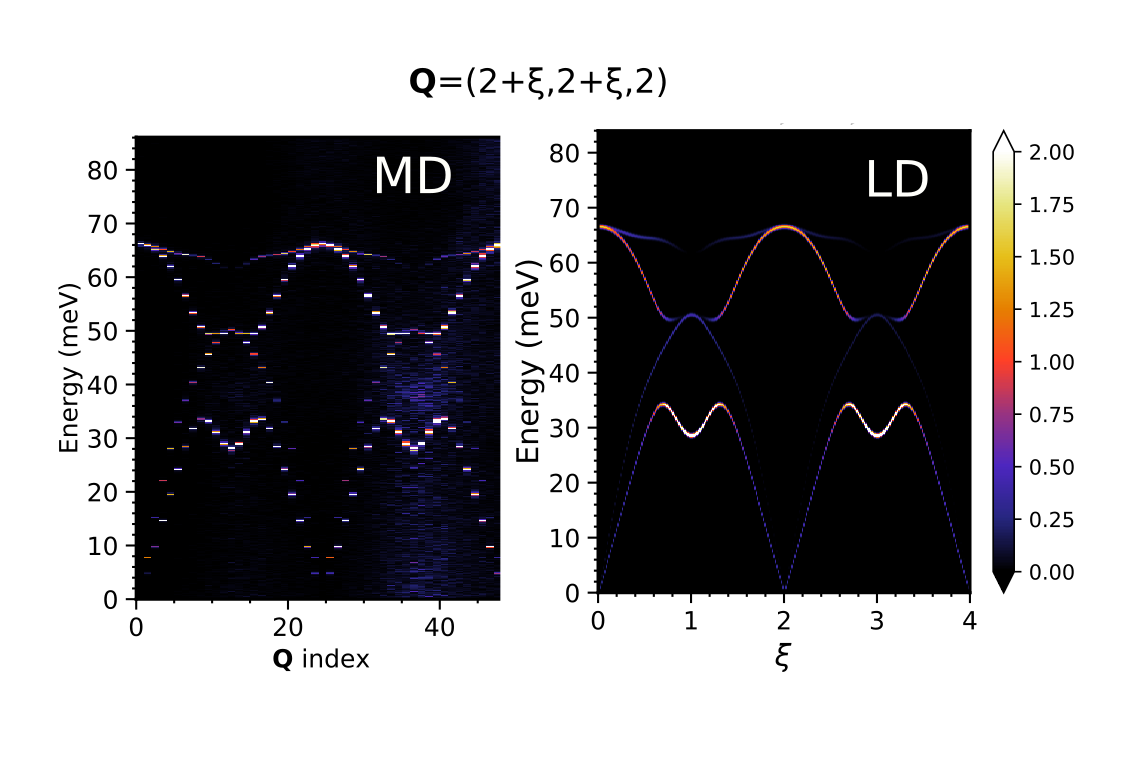
\includegraphics[width=\linewidth]{./figs/path_1.png}
        \caption{}
\label{fig:path_1}
\end{figure}

\begin{figure}
  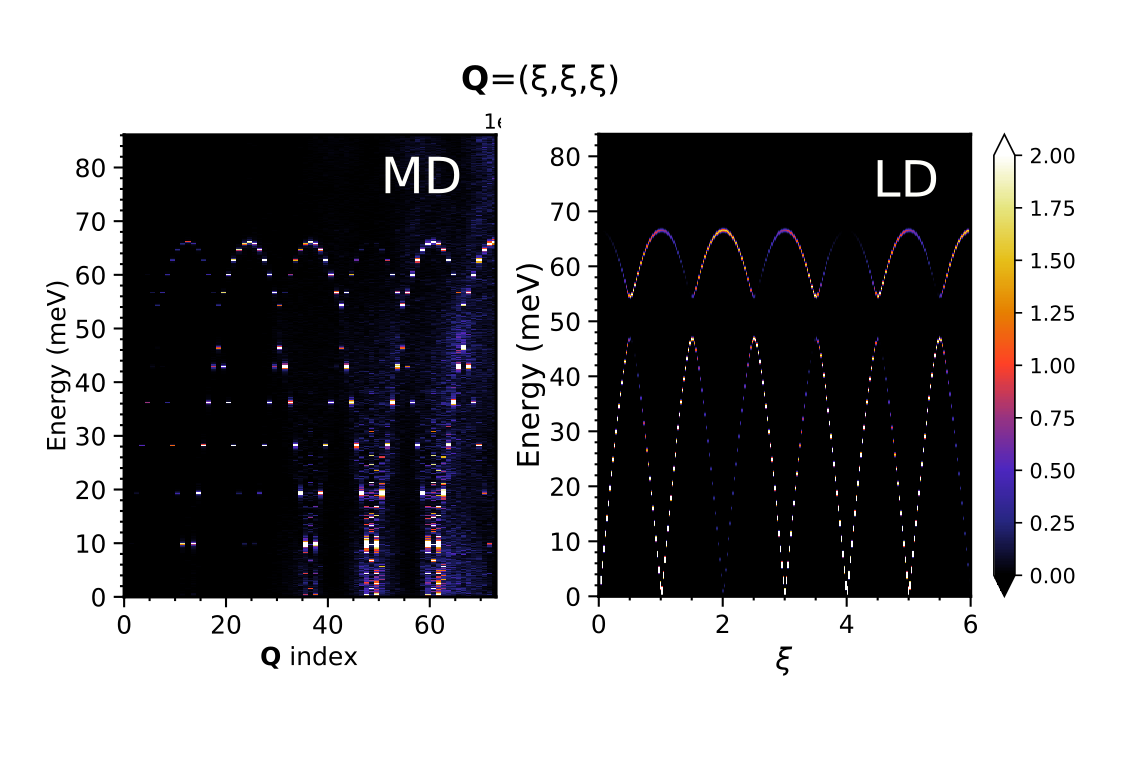
\includegraphics[width=\linewidth]{./figs/path_2.png}
        \caption{}
\label{fig:path_2}
\end{figure}

\begin{figure}
  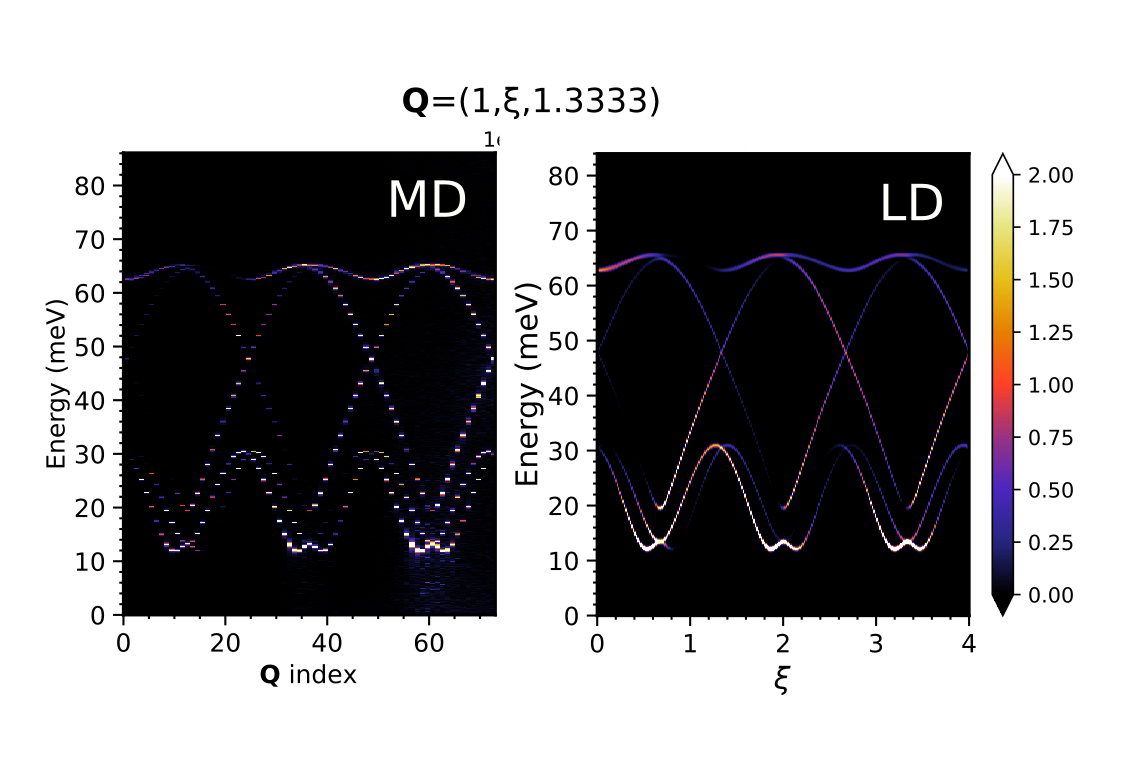
\includegraphics[width=\linewidth]{./figs/path_3.png}
        \caption{}
\label{fig:path_3}
\end{figure}

\begin{figure}
  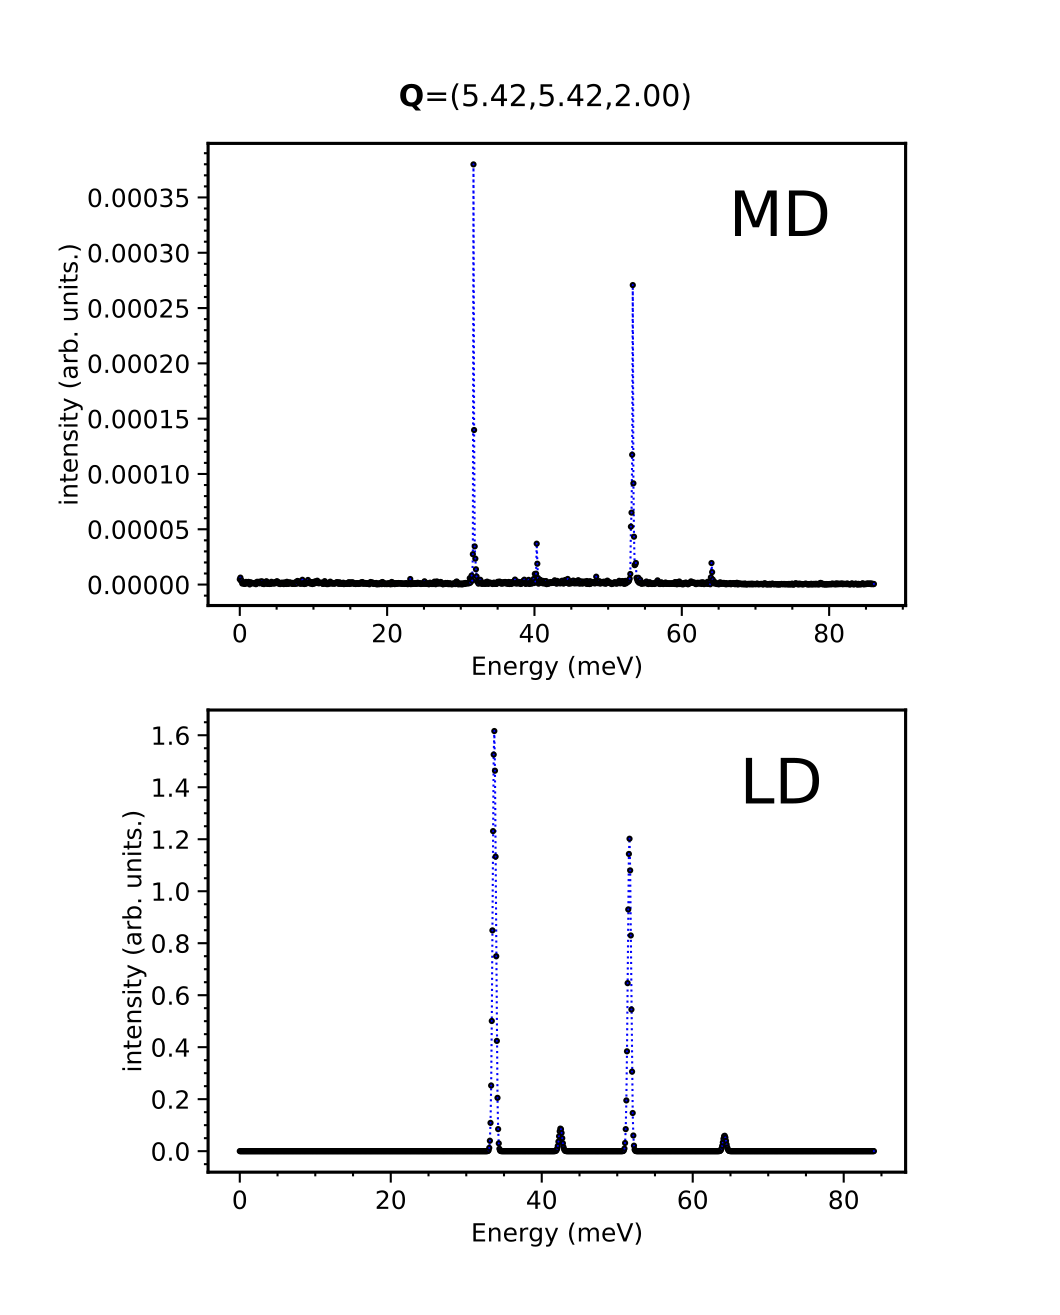
\includegraphics[width=\linewidth]{./figs/const_Q_validation.png}
        \caption{}
\label{fig:const_Q_validation}
\end{figure}


\bibliography{ref}

\end{document}

